\documentclass{article}
\usepackage{graphicx} % new way of doing eps files
\usepackage{listings} % nice code layout
\usepackage[usenames]{color} % color
\usepackage{float}
\definecolor{listinggray}{gray}{0.9}
\definecolor{graphgray}{gray}{0.7}
\definecolor{ans}{rgb}{1,0,0}
\definecolor{blue}{rgb}{0,0,1}
% \Verilog{title}{label}{file}
\newcommand{\Verilog}[3]{
  \lstset{language=Verilog}
  \lstset{backgroundcolor=\color{listinggray},rulecolor=\color{blue}}
  \lstset{linewidth=\textwidth}
  \lstset{commentstyle=\textit, stringstyle=\upshape,showspaces=false}
  \lstset{frame=tb}
  \lstinputlisting[caption={#1},label={#2}]{#3}
}


\author{Jiasen Zhou, Jon Johnston}
\title{Lab 8}

\begin{document}
\maketitle

\section{Executive Summary}
The purpose of this lab is to design and simulate the execute stage of the datapath. The execute stage is made up of the primary ALU for executing instructions, another ALU for branching, and control modules for their operation. This stage is responsible for performing the necessary arithmetic to execute instructions on data in registers and memory as well as branching. Mostly, this lab pertained to connecting modules created in earlier labs. After running the test for the module and comparing it to expected results, the lab proved to be successful.

\section{Test Report}
To verify operation of this module, this lab requires one test bench.  
\begin{enumerate}
	\item iExecute Test Bench
\end{enumerate}

\pagebreak

\begin{figure}[H]
	\begin{center}
		\caption{Expected Results of the iExecute test.}\label{fig:ert_iexecutetest}
		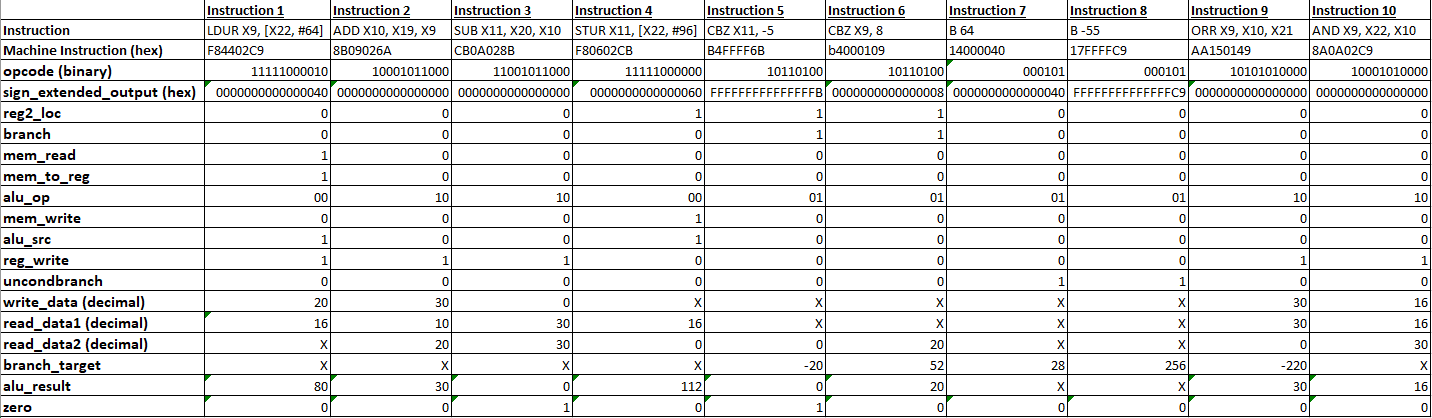
\includegraphics[width=1.0\textwidth]{../images/iExecuteExpected.png}
	\end{center}
\end{figure}

\begin{figure}[H]
	\begin{center}
		\caption{Timing diagram for the iExecute test.}\label{fig:iexecutetest}
		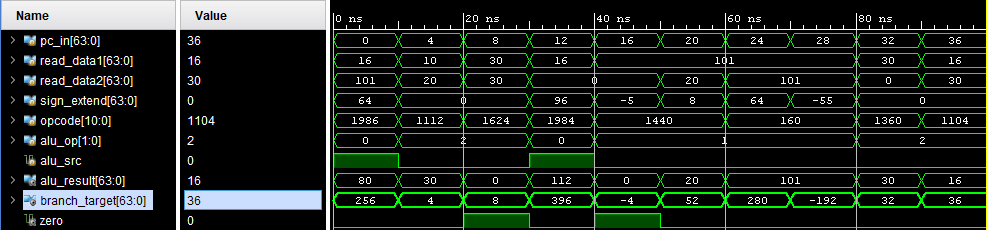
\includegraphics[width=1.0\textwidth]{../images/iExecuteSimulation.png}
	\end{center}
\end{figure}


\section{Code Appendix}
% The code appendix should include the test bench code and module code for this lab.
\Verilog{Verilog code for testing the iExecute module.}{code:regtest}{../code/3_execute/iExecute_test.v}
\Verilog{Verilog code for the iExecute module}{code:reg}{../code/3_execute/iExecute.v}
\end{document} 